\documentclass[11pt]{article}
\usepackage[table]{xcolor}
\usepackage{amsmath} 
\usepackage{graphicx}
\usepackage{subcaption}
\usepackage{sectsty}
\usepackage{amssymb}
 \usepackage{lipsum}
\usepackage{titlesec}
\usepackage{romannum}
\usepackage{enumitem}
\usepackage{mathtools}
\usepackage[super]{nth}
\usepackage{tikz}
\usepackage{listings}
\usepackage{pagecolor,lipsum}
\usepackage{color,soul}
\usepackage{xcolor}
\usepackage{hyperref}
\usepackage[T1]{fontenc}
\usepackage{textcomp}
\usepackage{float}
\usepackage{media9}
\usepackage[utf8]{inputenc}
\usepackage[T1]{fontenc}
\usepackage{parskip}

\definecolor{theWhite}{gray}{0.9}
\definecolor{theBlack}{gray}{0.0}
\definecolor{dkgreen}{rgb}{0,0.6,0}
\definecolor{gray}{rgb}{0.5,0.5,0.5}
\definecolor{mauve}{rgb}{0.58,0,0.82}
\definecolor{codegreen}{rgb}{0,0.6,0}
\definecolor{codegray}{rgb}{0.5,0.5,0.5}
\definecolor{codepurple}{rgb}{0.58,0,0.82}
\definecolor{backcolour}{rgb}{0.95,0.95,0.92}
\definecolor{orange}{RGB}{255,127,0}
\pagecolor{white}
\graphicspath{ {./images/} }
\setlength{\fboxsep}{1pt}


\lstdefinelanguage{Comment}{
  identifierstyle=\color{white},
  sensitive=false,
}

\lstdefinelanguage{HTML5}{
        language=html,
        sensitive=true, 
        alsoletter={<>=-},
        otherkeywords={
        % HTML tags
        <html>, <head>, 
        <title>, </title>, 
        <meta, />, </head>, 
        <body>, </body>, 
        <p>, </p>, 
        <div>, </div>, 
        <h1>, </h1>,
        <br>, 
        <ul>, </ul>, 
        <li>, </li>,
        <ol>, </ol>, 
        <img, />, 
        <video, </video>, 
        <canvas, \/canvas>, 
        <script>, </script>, 
      	</html>, <!, html>, 
	<style>, </style>, 
	><, 
	<div, 
	<strong>, </strong>, 
	<em>, </em>, 
	<a>, </a>, <a
        },  
        %ndkeywords={
        % General
        % =,
        % HTML attributes
        %charset=, id=, width=, height=,
        % CSS properties
        %border:, transform:, -moz-transform:, transition-duration:, transition-property:, transition-timing-function:
        %},  
        morecomment=[s]{<!--}{-->},
        %tag=[s]
}

\lstset{
    language={HTML5},
    backgroundcolor=\color{backcolour},
    basicstyle={\small\ttfamily},   
    frame=l,
    % Line numbers
    xleftmargin={0.5cm},
    numbers=left,
    stepnumber=1,
    firstnumber=1,
    numberfirstline=true,
    % Code design   
    numberstyle=\tiny\color{codegray},
    ndkeywordstyle=\color{codegreen}\bfseries,
    keywordstyle=\color{blue},
    commentstyle=\color{gray},
    stringstyle=\color{mauve},
    escapeinside={(*@}{@*)}, 
    % Code
    %alsodigit={.:;},
    %tabsize=2,
    %showtabs=false,
    %showspaces=false,
    %showstringspaces=false,
    %extendedchars=true,
    %breaklines=true,        
}

\newcommand*\circled[1]{\tikz[baseline=(char.base)]{
            \node[shape=circle,draw,inner sep=2pt] (char) {#1};}}
\setlength\parindent{0pt}
\setlist[itemize,1]{leftmargin=\dimexpr 26pt-.5in}

\sectionfont{\fontsize{12}{15}\selectfont}
\title{Introduction to Programming with Javascript}
\author{Qitian Liao}
\date{Aug 3, 2020} 
\usepackage[left=2cm, right=2cm, top=2cm]{geometry}
%\setlength\parindent{0pt}

\DeclarePairedDelimiter\abs{\lvert}{\rvert}
\DeclarePairedDelimiter\norm{\lVert}{\rVert}

\begin{document}
\begin{titlepage}
	\begin{center} 
	\line(1, 0){400}\\
	[0.25in]
	\huge{\bfseries Introduction to HTML} \\
	[2mm]
	\line(1, 0){300} \\
	[1.5cm]
	\textsc{\LARGE Qitian Liao} \\
	[0.5cm]
	\textsc{\large University of California, Berkeley} \\
	[15cm]
	\end{center}
	\begin{flushright}	
	\end{flushright}
\end{titlepage}

\thispagestyle{empty}
\newpage
\tableofcontents
\thispagestyle{empty}
\cleardoublepage
\setcounter{page}{1}
\def\Arg{\mathop{\operator@font Arg}\nolimits}
\pagenumbering{arabic}
\titleformat*{\section}{\Large\bfseries}
\titleformat*{\subsection}{\large\bfseries}
\titleformat*{\subsubsection}{\normalsize\bfseries}
\titleformat*{\paragraph}{\large\bfseries}
\titleformat*{\subparagraph}{\large\bfseries}
\newpage

\section{Introduction to HTML}
Now we will learn the basic structure of an HTML document.
\subsection{Introduction to HTML}
HTML is the skeleton of all web pages. It is often the first language learned by developers, marketers, and designers and is core to front-end development work. HTML provides structure to the content appearing on a website, such as images, text, or videos. Right-click on any page on the internet, choose “Inspect,” and we will see HTML in a panel of your screen. 

HTML stands for HyperText Markup Language:
\begin{itemize}[leftmargin = *]
\item A \textit{markup} language is a computer language that defines the structure and presentation of raw text.
\item In HTML, the computer can interpret \textit{raw text} that is wrapped in HTML elements.
\item \textit{HyperText} is text displayed on a computer or device that provides access to other text through links, also known as \textit{hyperlinks}. 
\end{itemize}
Learning HTML is the first step in creating websites, but even a bit of knowledge can help us inject code snippets into newsletter, blog or website templates. As we continue learning, we can layer HTML with CSS and JavaScript to create visually compelling and dynamic websites. Now, we are going to focus on how to add and modify basic content on a page, like text, images, and videos.

\subsection{HTML Anatomy}
HTML is composed of \textit{elements}. These elements structure the webpage and define its content. Let us take a look at how they are written.
\begin{figure}[H]
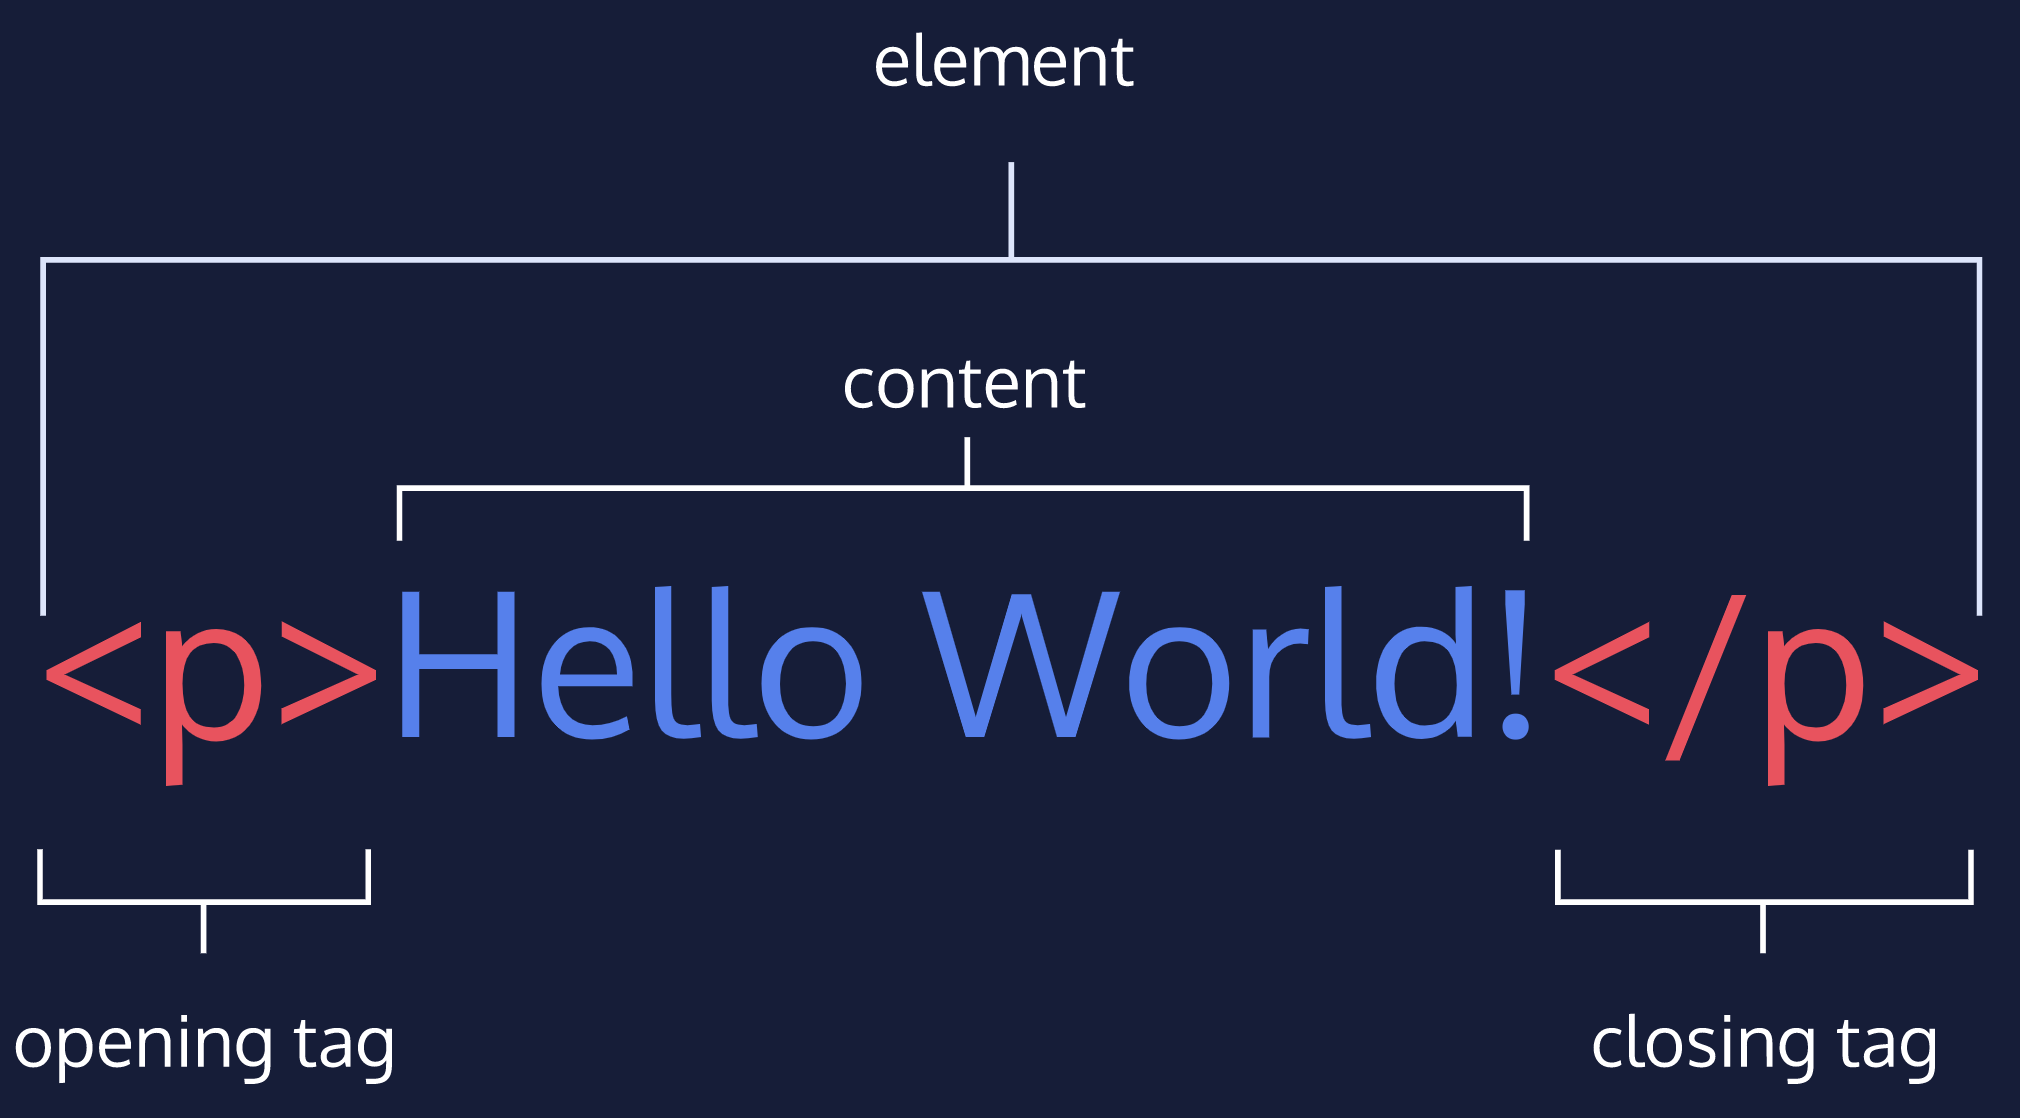
\includegraphics[scale = 0.2]{1_1}
\centering
\end{figure}
The diagram above displays an HTML paragraph element. As we can see, the paragraph element is made up of:
\begin{itemize}[leftmargin = *]
\item An \textit{opening tag} (\colorbox{lightgray}{<p>})
\item The content (“Hello World!” text)
\item A \textit{closing tag} (\colorbox{lightgray}{<$/$p>})
\end{itemize}
A \textit{tag} and the \textit{content} between it is called an HTML element. There are many tags that we can use to organize and display text and other types of content, like images. 

Let us quickly review each part of the element pictured:
\begin{itemize}[leftmargin = *]
\item HTML element (or simply, element) — a unit of content in an HTML document formed by HTML tags and the text or media it contains.
\item HTML Tag — the element name, surrounded by an opening (\colorbox{lightgray}{<}) and closing (\colorbox{lightgray}{>}) angle bracket. 
\item Opening Tag — the first HTML tag used to start an HTML element. The tag type is surrounded by opening and closing angle brackets.
\item Content — The information (text or other elements) contained between the opening and closing tags of an HTML element.
\item Closing tag — the second HTML tag used to end an HTML element. Closing tags have a forward slash (\colorbox{lightgray}{$/$}) inside of them, directly after the left angle bracket.
\end{itemize}

\subsection{The Body}
One of the key HTML elements we use to build a webpage is the \textit{body} element. Only content inside the opening and closing body tags can be displayed to the screen. Here is what opening and closing body tags look like:
\begin{lstlisting}
<body>

</body>
\end{lstlisting}
Once the file has a body, many different types of content – including text, images, and buttons – can be added to the body.
\begin{lstlisting}
<body>
  <p>What's up, doc?</p>
</body>
\end{lstlisting}

\subsection{HTML Structure}
HTML is organized as a collection of family tree relationships. As you saw in the last exercise, we placed \colorbox{lightgray}{<p>} tags within \colorbox{lightgray}{<body>} tags. When an element is contained inside another element, it is considered the \textit{child} of that element. The child element is said to be \textit{nested} inside of the \textit{parent} element.
\begin{lstlisting}
<body>
  <p>This paragraph is a child of the body</p>
</body>
\end{lstlisting}
In the example above, the \colorbox{lightgray}{<p>} element is nested inside the \colorbox{lightgray}{<body>} element. The \colorbox{lightgray}{<p>} element is considered a child of the \colorbox{lightgray}{<body>} element, and the \colorbox{lightgray}{<body>} element is considered the parent. Notice that we have added two spaces of indentation (using the \framebox[1.1\width]{space} bar) for better readability. 

Since there can be multiple levels of nesting, this analogy can be extended to grandchildren, great-grandchildren, and beyond. The relationship between elements and their ancestor and descendent elements is known as \textit{hierarchy}. 

Let us consider a more complicated example that uses some new tags: 
\begin{lstlisting}
<body>
  <div>
    <h1>Sibling to p, but also grandchild of body</h1>
    <p>Sibling to h1, but also grandchild of body</p>
  </div>
</body>
\end{lstlisting}
In this example, the \colorbox{lightgray}{<body>} element is the parent of the \colorbox{lightgray}{<div>} element. Both the \colorbox{lightgray}{<h1>} and \colorbox{lightgray}{<p>} elements are children of the \colorbox{lightgray}{<div>} element. Because the \colorbox{lightgray}{<h1>} and \colorbox{lightgray}{<p>} elements are at the same level, they are considered siblings and are both grandchildren of the \colorbox{lightgray}{<body>} element.

Understanding HTML hierarchy is important because child elements can inherit behavior and styling from their parent element. We will learn more about webpage hierarchy when you start digging into CSS.

\subsection{Headings}
Headings in HTML are similar to headings in other types of media. For example, in newspapers, large headings are typically used to capture a reader’s attention. Other times, headings are used to describe content, like the title of a movie or an educational article.

HTML follows a similar pattern. In HTML, there are six different \textit{headings}, or \textit{heading elements}. Headings can be used for a variety of purposes, like titling sections, articles, or other forms of content.

The following is the list of heading elements available in HTML. They are ordered from largest to smallest in size.
\begin{enumerate}[leftmargin = *]
\item \colorbox{lightgray}{<h1>} — used for main headings. All other smaller headings are used for subheadings.
\item \colorbox{lightgray}{<h2>}
\item \colorbox{lightgray}{<h3>}
\item \colorbox{lightgray}{<h4>}
\item \colorbox{lightgray}{<h5>}
\item \colorbox{lightgray}{<h6>}
\end{enumerate}
The following example code uses a headline intended to capture a reader’s attention. It uses the largest heading available, the main heading element:
\begin{lstlisting}
<h1>BREAKING NEWS</h1>
\end{lstlisting}

\subsection{Divs}
One of the most popular elements in HTML is the \colorbox{lightgray}{<div>} element. \colorbox{lightgray}{<div>} is short for “division” or a container that divides the page into sections. These sections are very useful for grouping elements in your HTML together.
\begin{lstlisting}
<body>
  <div>
    <h1>Why use divs?</h1>
    <p>Great for grouping elements!</p>
  </div>
</body>
\end{lstlisting}
\colorbox{lightgray}{<div>}s can contain any text or other HTML elements, such as links, images, or videos. Remember to always add two spaces of indentation when you nest elements inside of \colorbox{lightgray}{<div>}s for better readability.

\subsection{Attributes}
If we want to expand an element’s tag, we can do so using an \textit{attribute}. Attributes are content added to the opening tag of an element and can be used in several different ways, from providing information to changing styling. Attributes are made up of the following two parts:
\begin{itemize}[leftmargin = *]
\item The \textit{name} of the attribute
\item The \textit{value} of the attribute
\end{itemize}
One commonly used attribute is the \colorbox{lightgray}{id}. We can use the \colorbox{lightgray}{id} attribute to specify different content (such as \colorbox{lightgray}{<div>}s) and is really helpful when you use an element more than once. \colorbox{lightgray}{id}s have several different purposes in HTML, but for now, we will focus on how they can help us identify content on our page.

When we add an \colorbox{lightgray}{id} to a \colorbox{lightgray}{<div>}, we place it in the opening tag:
\begin{lstlisting}
<div id="intro">
  <h1>Introduction</h1>
</div>
\end{lstlisting}

\subsection{Displaying Text}
If you want to display text in HTML, you can use a \textit{paragraph} or \textit{span}:
\begin{itemize}[leftmargin = *]
\item \textit{Paragraphs} (\colorbox{lightgray}{<p>}) contain a block of plain text.
\item \colorbox{lightgray}{<span>} contains short pieces of text or other HTML. They are used to separate small pieces of content that are on the same line as other content.
\end{itemize}
Take a look at each of these elements in action below:
\begin{lstlisting}
<div>
  <h1>Technology</h1>
</div>
<div>
  <p><span>Self-driving cars</span> are anticipated to 
  replace up to 2 million jobs over the next two decades.</p>
</div>
\end{lstlisting}
In the example above, there are two different \colorbox{lightgray}{<div>}. The second \colorbox{lightgray}{<div>} contains a \colorbox{lightgray}{<p>} with \\
\colorbox{lightgray}{<span>Self-driving cars</span>}. This \colorbox{lightgray}{<span>} element separates “Self-driving cars” from the rest of the text in the paragraph.

It is best to use a \colorbox{lightgray}{<span>} element when you want to target a specific piece of content that is inline, or on the same line as other text. If you want to divide your content into blocks, it is better to use a \colorbox{lightgray}{<div>}.

\subsection{Styling Text}
You can also style text using HTML tags. The \colorbox{lightgray}{<em>} tag emphasizes text, while the \colorbox{lightgray}{<strong>} tag highlights important text.

Later, when we begin to style websites, we will decide how you want browsers to display content within \colorbox{lightgray}{<em>} and \colorbox{lightgray}{<strong>} tags. Browsers, however, have built-in style sheets that will generally style these tags in the following ways:
\begin{itemize}[leftmargin = *]
\item The \colorbox{lightgray}{<em>} tag will generally render as italic emphasis.
\item The \colorbox{lightgray}{<strong>} will generally render as bold emphasis.
\end{itemize}
Take a look at each style in action:
\begin{lstlisting}
<p><strong>The Nile River</strong> is the <em>longest</em> 
river in the world, measuring over 6,850 kilometers long 
(approximately 4,260 miles).</p>
\end{lstlisting}
In this example, the \colorbox{lightgray}{<strong>} and \colorbox{lightgray}{<em>} tags are used to emphasize the text to produce the following:
\vspace{-3mm}
\par\noindent\rule{\textwidth}{0.2pt}
\textbf{The Nile River} is the \textit{longest} river in the world, measuring over 6,850 kilometers long (approximately 4,260 miles).
\vspace{-3mm}
\par\noindent\rule{\textwidth}{0.2pt}
As we can see, “The Nile River” is bolded and “longest” is in italics.

\subsection{Line Breaks}
The spacing between code in an HTML file does not affect the positioning of elements in the browser. If you are interested in modifying the spacing in the browser, you can use HTML’s \textit{line break} element: \colorbox{lightgray}{<br>}.

The line break element is unique because it is only composed of a starting tag. You can use it anywhere within your HTML code and a line break will be shown in the browser.
\begin{lstlisting}
<p>The Nile River is the longest river <br> in the world, 
measuring over 6,850 <br> kilometers long (approximately 
4,260 <br> miles).</p>
\end{lstlisting}
The code in the example above will result in an output that looks like the following:
\vspace{-3mm}
\par\noindent\rule{\textwidth}{0.2pt}
The Nile River is the longest river \\ 
in the world, measuring over 6,850 \\ 
kilometers long (approximately 4,260 \\
miles).
\vspace{-3mm}
\par\noindent\rule{\textwidth}{0.2pt}

\subsection{Unordered Lists}
In addition to organizing text in paragraph form, you can also display content in an easy-to-read list.

In HTML, you can use an \textit{unordered list} tag (\colorbox{lightgray}{<ul>}) to create a list of items in no particular order. An unordered list outlines individual list items with a bullet point.

The \colorbox{lightgray}{<ul>} element should not hold raw text and will not automatically format raw text into an unordered list of items. Individual list items must be added to the unordered list using the \colorbox{lightgray}{<li>} tag. The \colorbox{lightgray}{<li>} or list item tag is used to describe an item in a list.
\begin{lstlisting}
<ul>
  <li>Limes</li>
  <li>Tortillas</li>
  <li>Chicken</li>
</ul>
\end{lstlisting}
In the example above, the list was created using the \colorbox{lightgray}{<ul>} tag and all individual list items were added using \colorbox{lightgray}{<li>} tags.

The output will look like this:
\vspace{-3mm}
\par\noindent\rule{\textwidth}{0.2pt}
\begin{itemize}[leftmargin = 24pt]
\item Limes
\item Tortillas
\item Chicken
\end{itemize}
\vspace{-3mm}
\par\noindent\rule{\textwidth}{0.2pt}

\subsection{Ordered Lists}
\textit{Ordered lists} (\colorbox{lightgray}{<ol>}) are like unordered lists, except that each list item is numbered. They are useful when you need to list different steps in a process or rank items for first to last.

You can create the ordered list with the \colorbox{lightgray}{<ol>} tag and then add individual list items to the list using \colorbox{lightgray}{<li>} tags.
\begin{lstlisting}
<ol>
  <li>Preheat the oven to 350 degrees.</li>
  <li>Mix whole wheat flour, baking soda, and salt.</li>
  <li>Cream the butter, sugar in separate bowl.</li>
  <li>Add eggs and vanilla extract to bowl.</li>
</ol>
\end{lstlisting}
The output will look like this:
\vspace{-3mm}
\par\noindent\rule{\textwidth}{0.2pt}
\begin{enumerate}[leftmargin = 24pt]
\item Preheat the oven to 350 degrees.
\item Mix whole wheat flour, baking soda, and salt.
\item Cream the butter, sugar in separate bowl.
\item Add eggs and vanilla extract to bowl.
\end{enumerate}
\vspace{-3mm}
\par\noindent\rule{\textwidth}{0.2pt}

\subsection{Images}
All of the elements we have learned about so far (headings, paragraphs, lists, and spans) share one thing in common: they are composed entirely of text. What if we want to add content to our web page that is not composed of text, like images?

The \colorbox{lightgray}{<img>} tag allows us to add an image to a web page. Most elements require both opening and closing tags, but the \colorbox{lightgray}{<img>} tag is a self-closing tag. Note that the end of the \colorbox{lightgray}{<img>} tag has a forward slash \colorbox{lightgray}{/}. Self-closing tags may include or omit the final slash — both will render properly.
\begin{lstlisting}
<img src="image-location.jpg" (*@/@*)>
\end{lstlisting}
The \colorbox{lightgray}{<img>} tag has a required \textit{attribute} called \colorbox{lightgray}{src}. The \colorbox{lightgray}{src} attribute must be set to the image’s \textit{source}, or the location of the image. In this case, the value of \colorbox{lightgray}{src} must be the \textit{uniform resource locator} (URL) of the image. A URL is the web address or local address where a file is stored.

\subsection{Image Alts}
Part of being an exceptional web developer is making our site accessible to users of all backgrounds. In order to make the Web more inclusive, we need to consider what happens when assistive technologies such as screen readers come across image tags.

The \colorbox{lightgray}{alt} attribute, which means alternative text, brings meaning to the images on our sites. The \colorbox{lightgray}{alt} attribute can be added to the image tag just like the \colorbox{lightgray}{src} attribute. The value of \colorbox{lightgray}{alt} should be a description of the image.
\begin{lstlisting}
<img src="#" alt="A(*@ @*)field of yellow sunflowers" (*@/@*)>
\end{lstlisting}
The \colorbox{lightgray}{alt} attribute also serves the following purposes:
\begin{itemize}[leftmargin = *]
\item If an image fails to load on a web page, a user can mouse over the area originally intended for the image and read a brief description of the image. This is made possible by the description you provide in the \colorbox{lightgray}{alt} attribute.
\item Visually impaired users often browse the web with the aid of screen reading software. When you include the alt attribute, the screen reading software can read the image’s description out loud to the visually impaired user.
\item The alt attribute also plays a role in Search Engine Optimization (SEO), because search engines cannot “see” the images on websites as they crawl the internet. Having descriptive alt attributes can improve the ranking of your site.
\end{itemize}
If the image on the web page is not one that conveys any meaningful information to a user (visually impaired or otherwise), the \colorbox{lightgray}{alt} attribute should be left empty.

\subsection{Videos}
In addition to images, HTML also supports displaying videos. Like the \colorbox{lightgray}{<img>} tag, the \colorbox{lightgray}{<video>} tag requires a src attribute with a link to the video source. Unlike the \colorbox{lightgray}{<img>} tag however, the \colorbox{lightgray}{<video>} element requires an opening and a closing tag.
\begin{lstlisting}
<video src="myVideo.mp4" width="320" height="240" controls>
  Video not supported
</video>
\end{lstlisting}
In this example, the video source (\colorbox{lightgray}{src}) is \colorbox{lightgray}{myVideo.mp4}. The source can be a video file that is hosted alongside your webpage, or a URL that points to a video file hosted on another webpage.

After the \colorbox{lightgray}{src} attribute, the \colorbox{lightgray}{width} and \colorbox{lightgray}{height} attributes are used to set the size of the video displayed in the browser. The \colorbox{lightgray}{controls} attribute instructs the browser to include basic video controls: pause, play and skip.

The text, “Video not supported”, between the opening and closing video tags will only be displayed if the browser is unable to load the video.

\subsection{Review}
Let us review what we have learned in this chapter:
\begin{itemize}[leftmargin = *]
\item \textbf{HTML} stands for \textbf{H}yper\textbf{T}ext \textbf{M}arkup \textbf{L}anguage and is used to create the structure and content of a webpage.
\item Most HTML elements contain opening and closing tags with raw text or other HTML tags between them.
\item HTML elements can be nested inside other elements. The enclosed element is the child of the enclosing parent element.
\item Any visible content should be placed within the opening and closing \colorbox{lightgray}{<body>} tags.
\item Headings and sub-headings, \colorbox{lightgray}{<h1>} to \colorbox{lightgray}{<h6>} tags, are used to enlarge text.
\item \colorbox{lightgray}{<p>}, \colorbox{lightgray}{<span>} and \colorbox{lightgray}{<div>} tags specify text or blocks.
\item The \colorbox{lightgray}{<em>} and \colorbox{lightgray}{<strong>} tags are used to emphasize text.
\item Line breaks are created with the \colorbox{lightgray}{<br>} tag.
\item Ordered lists (\colorbox{lightgray}{<ol>}) are numbered and unordered lists (\colorbox{lightgray}{<ul>}) are bulleted.
\item Images (\colorbox{lightgray}{<img>}) and videos (\colorbox{lightgray}{<video>}) can be added by linking to an existing source.
\end{itemize}
Next, we will take the content that we have added to the website and transform it into an HTML document that is ready to go on the web.

\newpage
\section{HTML Document Standards}
Now we will learn how to set up a proper HTML Document, how to link to other pages, and how to format our code for readability.
\subsection{Preparing for HTML}
Now it is time to learn how to set up an HTML file. HTML files require certain elements to set up the document properly. We can let web browsers know that we are using HTML by starting our document with a \textit{document type declaration}.

The declaration looks like this:
\begin{lstlisting}
<!DOCTYPE html>
\end{lstlisting}
This declaration is an instruction, and it must be the first line of code in your HTML document. It tells the browser what type of document to expect, along with what version of HTML is being used in the document. For now, the browser will correctly assume that the \colorbox{lightgray}{html} in \colorbox{lightgray}{<!DOCTYPE html>} is referring to HTML5, as it is the current standard.

In the future, however, a new standard will override HTML5. To make sure your document is forever interpreted correctly, always include \colorbox{lightgray}{<!DOCTYPE html>} at the very beginning of your HTML documents.

Lastly, HTML code is always saved in a file with an \textbf{.html} extension.

\subsection{The <html> tag}
The \colorbox{lightgray}{<!DOCTYPE html>} declaration provides the browser with two pieces of information (the type of document and the HTML version to expect), but it does not actually add any HTML structure or content.

To create HTML structure and content, we must add opening and closing \colorbox{lightgray}{<html>} tags after declaring \colorbox{lightgray}{<!DOCTYPE html>}:
\begin{lstlisting}
<!DOCTYPE html>
<html>

</html>
\end{lstlisting}
Anything between the opening \colorbox{lightgray}{<html>} and closing \colorbox{lightgray}{</html>} tags will be interpreted as HTML code. Without these tags, it is possible that browsers could incorrectly interpret your HTML code.

\subsection{The Head}
So far we have done two things to set up the file properly:
\begin{itemize}[leftmargin = *]
\item Declared to the browser that your code is HTML with \colorbox{lightgray}{<!DOCTYPE html>}
\item Added the HTML element (\colorbox{lightgray}{<html>}) that will contain the rest of your code.
\end{itemize}
Now, let us also give the browser some information about the page itself. We can do this by adding a \colorbox{lightgray}{<head>} element.

The \colorbox{lightgray}{<head>} element is part of the HTML metaphor as the \colorbox{lightgray}{<body>} tag. It goes above the \colorbox{lightgray}{<body>} element.

The \colorbox{lightgray}{<head>} element contains the \textit{metadata} for a web page. Metadata is information about the page that is not displayed directly on the web page. Unlike the information inside of the \colorbox{lightgray}{<body>} tag, the metadata in the head is information about the page itself. 

The opening and closing head tags typically appear as the first item after our first HTML tag:
\begin{lstlisting}
<head>
</head>
\end{lstlisting}

\subsection{Page Titles}
Let us investigate what kind of metadata about the web page can the \colorbox{lightgray}{<head>} element contain.

A browser’s tab displays the \textit{title} specified in the \colorbox{lightgray}{<title>} tag. The \colorbox{lightgray}{<title>} tag is always inside of the \colorbox{lightgray}{<head>}.
\begin{lstlisting}
<!DOCTYPE html>
<html>
  <head>
    <title>My Coding Journal</title>
  </head>
</html>
\end{lstlisting}
If we were to open a file containing the HTML code in the example above, the browser would display the words \colorbox{lightgray}{My Coding Journal} in the title bar (or in the tab’s title).

\subsection{Where Does the Title Appear?}
Our title would appear as depicted in the diagram below.
\begin{figure}[H]
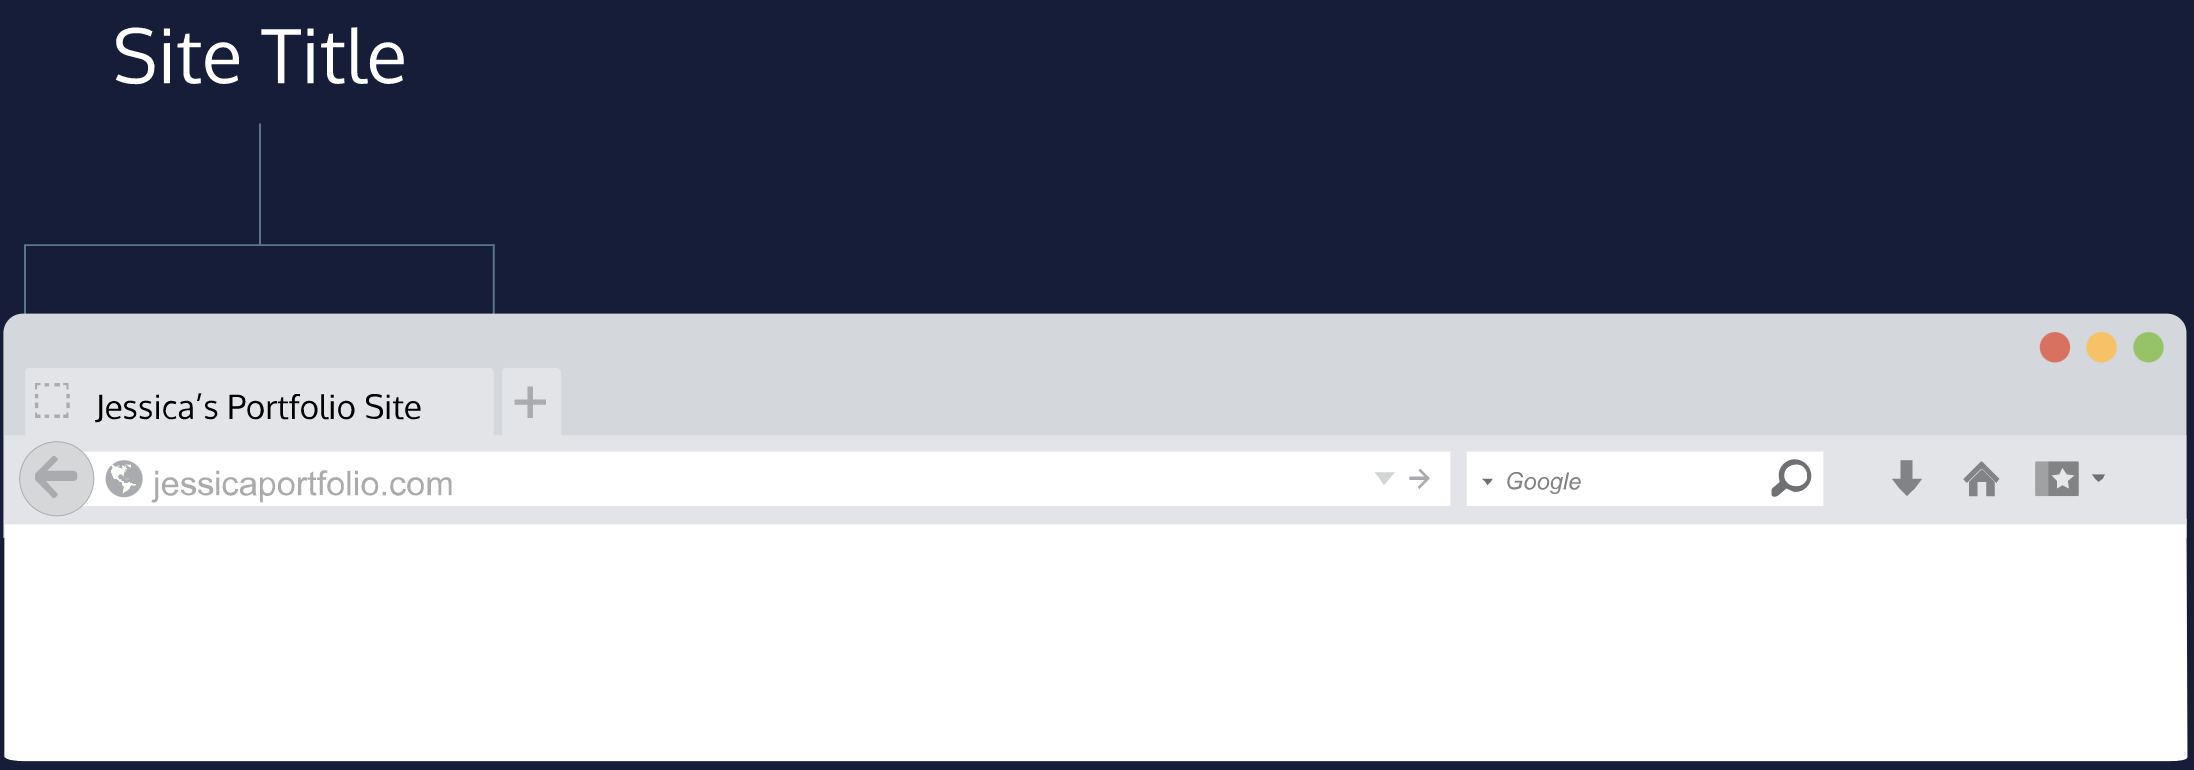
\includegraphics[scale = 0.4]{1_2}
\centering
\end{figure}
So far, we have learned about:
\begin{itemize}[leftmargin = *]
\item \colorbox{lightgray}{<!DOCTYPE html>}, the declaration specifying the version of HTML for the browser
\item The \colorbox{lightgray}{<html>} tags that enclose all of your HTML code
\item The \colorbox{lightgray}{<head>} tag that contains the metadata of a webpage, such as its \colorbox{lightgray}{<title>}
\end{itemize}
Next, we will learn about new types of elements that go inside the body.

\subsection{Linking to Other Web Pages}
One of the powerful aspects of HTML (and the Internet), is the ability to \textit{link} to other web pages.

We can add links to a web page by adding an \textit{anchor} element \colorbox{lightgray}{<a>} and including the text of the link in between the opening and closing tags.
\begin{lstlisting}
<a>This Is A Link To Wikipedia</a>
\end{lstlisting}
Technically, the link in the example above is incomplete. The link above cannot work because there is no URL that will lead users to the actual Wikipedia page. 

The anchor element in the example above is incomplete without the \colorbox{lightgray}{href} attribute. This attribute stands for \textit{hyperlink reference} and is used to link to a \textit{path}, or the address to where a file is located (whether it is on your computer or another location). The paths provided to the \colorbox{lightgray}{href} attribute are often URLs.
\begin{lstlisting}
<a href="https://www.wikipedia.org/">This Is A Link To Wikipedia</a>
\end{lstlisting}
In the example above, the \colorbox{lightgray}{href} attribute has been set to the value of the URL \colorbox{lightgray}{https://www.wikipedia.org/}. The example now shows the correct use of an anchor element.

When reading technical documentation, we may come across the term \textit{hyperlink}. This is simply the technical term for link, and these terms are often used interchangeably.

\subsection{Opening Links in a New Window}
Have you ever clicked on a link and observed the resulting web page open in a new browser window? If so, you can thank the \colorbox{lightgray}{<a>} element’s \colorbox{lightgray}{target} attribute.

The \colorbox{lightgray}{target} attribute specifies how a link should open.

It is possible that one or more links on your web page link to an entirely different website. In that case, you may want users to read the linked website, but hope that they return to your web page. This is exactly when the \colorbox{lightgray}{target} attribute is useful.

For a link to open in a new window, the \colorbox{lightgray}{target} attribute requires a value of \colorbox{lightgray}{\_blank}. The \colorbox{lightgray}{target} attribute can be added directly to the opening tag of the anchor element, just like the \colorbox{lightgray}{href} attribute.
\begin{lstlisting}
<a href="https://en.wikipedia.org/wiki/Brown_bear" 
target="_blank">The Brown Bear</a>
\end{lstlisting}
In the example above, setting the \colorbox{lightgray}{target} attribute to "\colorbox{lightgray}{\_blank}" instructs the browser to open the relevant Wikipedia page in a new window.

In this exercise, we have used the terminology “open in a new window.” It is likely that you are using a modern browser that opens up websites in new \textit{tabs}, rather than new windows. Before the advent of browsers with tabs, additional browser windows had to be opened to view more websites. The \colorbox{lightgray}{target="\_blank"} attribute, when used in modern browsers, will open new websites in a new tab.

\subsection{Linking to Relative Page}
Thus far we have learned how to link to external web pages. Many sites also link to internal web pages like Home, About, and Contact.

Before we learn how to link between internal pages, let us establish where our files are stored. When making multi-page static websites, web developers often store HTML files in the root directory, or a main folder where all the files for the project are stored. As the size of the projects you create grows, you may use additional folders within the main project folder to organize your code.
\begin{lstlisting}[basicstyle=\small\ttfamily\color{theWhite}, backgroundcolor = \color{theBlack}, language = Comment]
project-folder/
|__ about.html
|__ contact.html
|__ index.html
\end{lstlisting}
The example above shows three different files — \textbf{about.html}, \textbf{contact.html}, and \textbf{index.html} in one folder.

HTML files are often stored in the same folder, as shown in the example above. If the browser is currently displaying \textbf{index.html}, it also knows that \textbf{about.html} and \textbf{contact.html} are in the same folder. Because the files are stored in the same folder, we can link web pages together using a \textit{relative path}.
\begin{lstlisting}
<a href="./contact.html">Contact</a>
\end{lstlisting}
In this example, the \colorbox{lightgray}{<a>} tag is used with a relative path to link from the current HTML file to the \colorbox{lightgray}{contact.html} file in the same folder. On the web page, \colorbox{lightgray}{Contact} will appear as a link.

A relative path is a filename that shows the path to a \textit{local file} (a file on the same website, such as \colorbox{lightgray}{./index.htm}l) versus an absolute path (a full URL, like \colorbox{lightgray}{https://www.codecademy.com/learn/learn-html} which is stored in a different folder). The \colorbox{lightgray}{./} in \colorbox{lightgray}{./index.html} tells the browser to look for the file in the current folder.

\subsection{Linking At Will}
You have probably visited websites where not all links were made up of text. Maybe the links you clicked on were images or some other form of content.

So far, we have added links that were made up of only text, like the following:
\begin{lstlisting}
<a href="https://en.wikipedia.org/wiki/Opuntia"
target="_blank">Prickly Pear</a>
\end{lstlisting}
Text-only links, however, would significantly decrease our flexibility as web developers.

Thankfully, HTML allows us to turn nearly any element into a link by wrapping that element with an anchor element. With this technique, it is possible to turn images into links by simply wrapping the \colorbox{lightgray}{<img>} element with an \colorbox{lightgray}{<a>} element.
\begin{lstlisting}
<a href="https://en.wikipedia.org/wiki/Opuntia" 
target="_blank">(*@@*)<img
src="https://www.Prickly_Pear_Closeup.jpg" alt="A(*@ @*)red 
prickly(*@ @*)pear fruit"/></a>
\end{lstlisting}
In the example above, an image of a prickly pear has been turned into a link by wrapping the outside of the \colorbox{lightgray}{<img>} element with an \colorbox{lightgray}{<a>} element.

\subsection{Linking to Same Page}
At this point, we have all the content we want on our page. Since we have so much content, it does not all fit on the screen. How do we make it easier for a user to jump to different portions of our page?

When users visit our site, we want them to be able to click a link and have the page automatically scroll to a specific section.

In order to link to a target on the same page, we must give the target an \textit{id}, like this:
\begin{lstlisting}
<p id="top">This is the top of the page!</p>
<h1 id="bottom">This is the bottom! </h1>
\end{lstlisting}
In this example, the \colorbox{lightgray}{<p>} element is assigned an \colorbox{lightgray}{id} of “top” and the \colorbox{lightgray}{<h1>} element is assigned “bottom.” An \colorbox{lightgray}{id} can be added to most elements on a webpage.

An \colorbox{lightgray}{id} should be descriptive to make it easier to remember the purpose of a link. The target link is a string containing the \colorbox{lightgray}{\#} character and the target element’s \colorbox{lightgray}{id}.
\begin{lstlisting}
<ol>
  <li><a href="#top">Top</a></li>
  <li><a href="#bottom">Bottom</a></li>
</ol>
\end{lstlisting}
In the example above, the links to \colorbox{lightgray}{<p id="top">} and \colorbox{lightgray}{<h1 id="bottom">} are embedded in an ordered list. These links appear in the browser as a numbered list of links. An \colorbox{lightgray}{id} is especially helpful for organizing content belonging to a \colorbox{lightgray}{div}.











\end{document}
